\documentclass[11pt]{article}

\usepackage{tex/STC}

\usepackage[sorting=none]{biblatex}
\addbibresource{STC.bib}

%Document
\begin{document}

\title{STC Drift-Time Relation\\\normalsize Computing Project}
\author{Alex Hergenhan\\CID: 0604432}
\maketitle

This report outlines a program written to study the drift-time relationship for gasses in the Small Prototype Test Chamber (STC) for the ALEPH Inner Tracking Chamber (ITC). The git repository for this project can be found at \href{https://github.com/amh-137/STC-drift-time}{https://github.com/amh-137/STC-drift-time}.

\section{Introduction}
\label{sec:intro}

\subsection{Setup}
\label{sec:setup}
A \texttt{make} file is included to compile the program, or it can be compiled with the command\\

\texttt{g++ src/main.cpp src/event.cpp src/event-helpers.cpp -o STC -std=c++17 -Wall `root-config --cflags` `root-config --libs`}\\

A separate script, \texttt{setup.sh} is included for building the folder structure (\texttt{data/}, \texttt{plots/ev-display/}). Please run this once, and move both \texttt{singletrack.raw} and \texttt{manytracks.raw} into the data folder. Setup and running should therefore be:
\begin{verbatim}
    $ git clone git@github.com:amh-137/STC-drift-time.git && cd STC-drift-time
    $ source setup.sh
    $ cp /path/to/singletrack.raw data/ && cp path/to/manytracks.raw data/
    $ make      # or g++ ....
    $ ./STC
\end{verbatim}
Aternitively, you can use the zipped file I emailed, but please still move the data to \texttt{data/}. All C++ code is in the \texttt{src/} folder. I have left the \texttt{tex/} and \texttt{py-tests/} folders, but none of my final results are from python scripts. The program does not utilise any python, only C++, these where just for testing (and writing this report).

\section{Program Structure \& Design}
\label{sec:program}
The program is structured as follows:
\begin{itemize}
    \item \texttt{main.cpp} - The main file that reads the data and calls the functions.
    \item \texttt{circle.h}, \texttt{line.h}, \texttt{hit.h} - Contains the structs used.
    \item \texttt{event.h}, \texttt{event.cpp} - The main event class - stores 8 hits and associated information, with event processing methods.
    \item \texttt{event-helpers.h}, \texttt{event-helpers.cpp} - Helper functions for the event class.
\end{itemize}


I outline a pseudocode for the program:
\begin{verbatim}
    while data:
        read 16 bytes from file
        create EVENT object with 8 HITS
        get V with minimisation
        get THETA
    
    bin V, THETA in histograms
    fit histograms
    return results
\end{verbatim}
An initial mock-up of the program was written in C++, (as can be seen in early commits to the GitHub) however it became challenging to test new ideas due to my comparative unfamiliarity with \texttt{ROOT}. I therefore switched to Python, testing ideas, geometry, and minimisation algorithms in notebooks in the \texttt{py-test} directory. With a working implementation, I translated with back to C++, hoping the compiled program would be faster. This was not the case with simple gradient descent, so I switched back to python to study and optimise the loss function. I moved from sum of distances to sum of squares of distances, and then to the secant method for faster minimisation. This was then translated back to C++ for the final implementation.

\section{Implimentation}
\label{sec:implimentation}



\subsection{Reading Data}
\label{sec:reading}
The file is opened and 16 bytes are read as an array of \text{chars}. These are 8 bit objects - each event is 16 bits. We therefore join two chars to form a \texttt{uint\_16t}, and perform bitwise operations on this 16 bit type to extract the layer, wire, and TDC information. However, before we recast the \texttt{char} as a \texttt{uint\_16t}, we must first cast each \texttt{char} to an \texttt{unsinged char}. This prevents mix up in bit manipulation when the most significant bit is 1. Bit shifting, and bitwise logic with masks is used to extract the data from the 16 bit \texttt{uint\_16t}, and store it in a struct \text{hit}. An array of size 8 \texttt{hit} stores the data for one event.\\


I utilize a minimisation algorithm with some basic geometry to find the velocities of ionisation electrons. This works as follows:
\begin{itemize}
    \item The two largest circles by TDC time are picked $c_1$ and $c_2$.
    \item The four tangents for these two circles are calculated using \texttt{get\_two\_circle\_tangent()}.
    \item The sum of the squares of the distances to the other 6 circles are found (the distance to the two largest circles is zero, as these are tangents).
    \item The radii of the circles are varied by multiplying by a constant factor, $v$ and the sum of the squares of the distances is recalculated.
\end{itemize}
The factor $v$ is varied until the sum of the squares of the distances is minimised. This is the velocity of the ionisation electrons.

\subsection{Tangents \& Circle - Line Distances}
\label{sec:tangents}
We define circles and lines by their equations
\begin{equation}
    (x - x^0_i)^2 + (y - y^0_i)^2 = r^2
    \label{eq:circle}
\end{equation}
\begin{equation}
    ax + by + c = 0,
    \label{eq:line}
\end{equation}
The parameters of these equations ($a$, $b$, $c$, $x_0$, $y_0$, $r$) are stored in the structs \texttt{line} and \texttt{circle}. The tangents are therefore \cite{circle-tangents} lines with
\begin{equation}\label{eq:tange/nts}
\begin{split}
    a &= \frac{\Delta x^0  \Delta r + d\Delta y^0}{(\Delta x^0)^2 + (\Delta y^0)^2}\\%\frac{x^0_1(r_1-r_2) + y^0_1((x^0_1)^2 + (x^0_1)^2-(r_1 - r_2)^2)}{(x^0_1)^2 + (x^0_1)^2}\\
    b &= \frac{\Delta y^0 \Delta r - d\Delta x^0}{(\Delta x^0)^2 + (\Delta y^0)^2}\\
    c &= r_1 - x^0_1a - y^0_1b
\end{split}
\end{equation}
where $\Delta x^0 = x^0_2 - x^0_1$, $\Delta y^0 = x^0_2 - y^0_1$, $\Delta r=r_2 - r_1$and $d=\sqrt{(\Delta (x^0)^2 + (\Delta y^0)^2-(\Delta r)^2}$. Note that the four tangents are from the four combinations of fliping the signs of $r_1$ and $r_2$. Finally, the distance between the $i$th circle and a line is given by
\begin{equation}
    d_i = \frac{|{ax^0_i + by^0_i + c}|}{\sqrt{a^2 + b^2}}.
    \label{eq:dist}
\end{equation}

\subsection{Minimisation}
\label{sec:minimisation}
The function we minimise is defined as
\begin{equation}
    L = \sum\limits_{\substack{i=1 \\ i\neq c_1, c_2}}^{8} d_i^2.
    \label{eq:loss}
\end{equation}
Initially, this was minimised with gradient descent (Appendix \ref{app:gradient-descent}). Gradient descent, however, was extremely slow, so we switched to the secant method for minimisation. The secant method is an algorithm that uses the secant line to find the root of a function $f(x)$ \cite{secant-history}. It is defined as 
\begin{equation}
    x_{k+1} = x_k - \frac{x_k - x_{k-1}}{f(x_k)-f(x_{k-1})} f(x_k).
    \label{eq:secant}
\end{equation}
Here, $x_k$ is our variable at step $k$, while $f(x_k)$ is the function we want to find the root of at step $k$. In this program, we use a modified verion of the secant function replaces $f(x_k)$ with $f'(x_k)$ (the derivative of $f(x)$). This modifies the secant method to a minimsation algorithm, instead of a root finding algorithm \cite{secant-minimsation}. This is implimented in the function \texttt{secant\_minimise()} as
\begin{equation}
    v_{k+1} = v_k - \frac{f'(v_k)}{f'(v_k) - f'(v_{k-1})}(v_k - v_{k-1}).
\end{equation}

While the program is running, arrays of doubles store the values of $v$ and $\theta$. To reduce memory usage, these arrays are of a fixed size $10^4$. Therefore, every $10^4$ events, the histograms for $v$ and $\theta$ are filled, and the array is reused for the next batch of events.

\section{Results}
\label{sec:results}
The program runs in $\approx 1$ minuite on my laptop. A fitted histogram for velocity \autoref{fig:vel} and angle \autoref{fig:angle} are produced. The program can also draw fitted events. This is done by passing the draw frequency as a parameter when running the program e.g
\begin{verbatim}
    $ ./STC 100000
\end{verbatim}
will draw every $100000^\text{th}$ event. By default, the program does not draw any events. The outputs are stored in \texttt{plots/ev-display/} and \autoref{fig:ev-display} shows an example.


\begin{figure}
\begin{subfigure}[h]{0.49\linewidth}
    \centering
    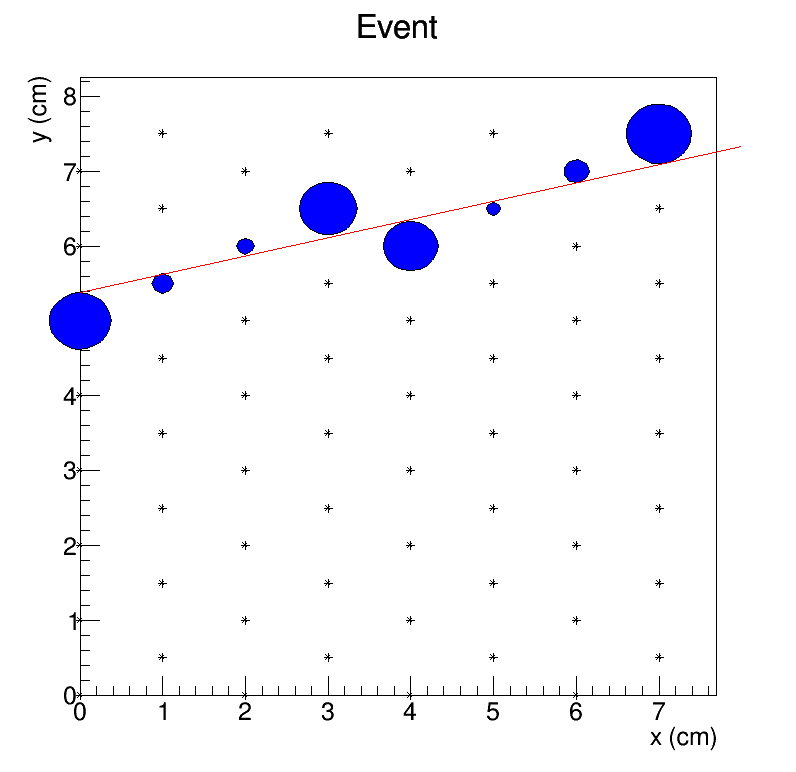
\includegraphics[width=1.0\linewidth]{tex/secant-10004.png}
\end{subfigure}
\begin{subfigure}[h]{0.49\linewidth}
    \centering
    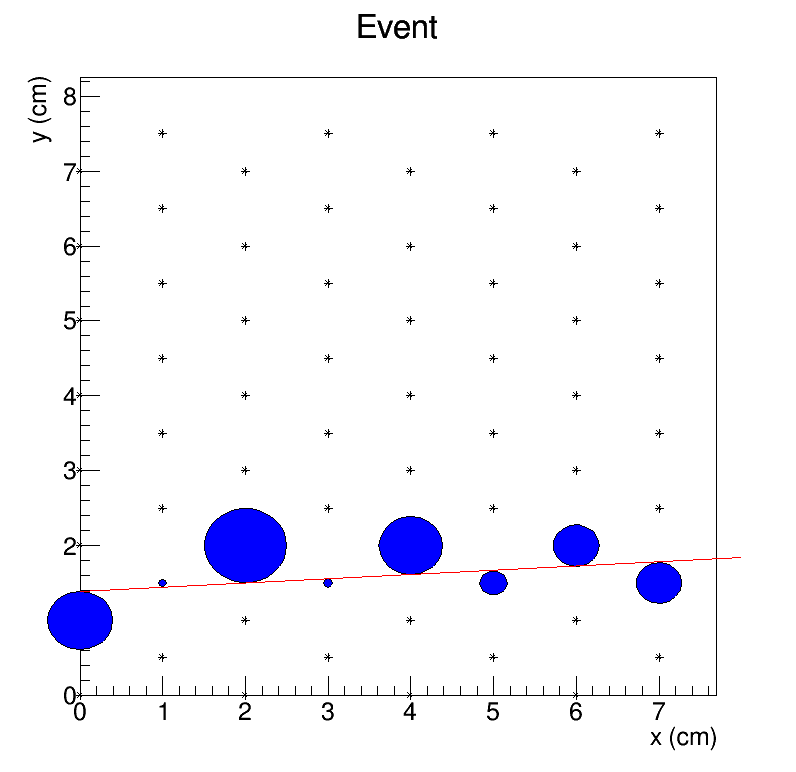
\includegraphics[width=1.0\linewidth]{tex/secant-300004.png}
\end{subfigure}
    \caption{(Left) display of event 10000. (Right) display of event 300000.}
\label{fig:ev-display}
\end{figure}

\section{Conclusion}
\label{sec:conclusion}
My results

I acknowledge that the program written has a far worse performance than others more geometric solutions. However, I did not want to just "copy" the best solution found - I built this solution myself, with minimal input from others. Getting to write and implement a minimisation of a function is something I have wanted to do for a while - I usually just use a library - so I stuck with this method for as long as possible. I am therefore pleased with my results, although I understand that the results will be worse than other students. I am particularly happy with the performance increases I achieved through optimisation of the minimisation procedure.

To improve the results and performance, I would switch to the method that involves finding the intersection points of the tangents of $N$ circles, and fitting a line to these points with simple linear regression. By repeating this linear regression and removing outliers, the path of the particle can be found, and hence the velocity can be found. To improve my method, I would try to calculate an analytic solution for the derivative, or use multi-threading to increase performance, which would allow for minimisations with a greater search depth.

\section{Acknowledgements}
\label{sec:acknowledgements}
Thanks to Calvin Dyson for his recommendation of the secant method for minimisation. Thanks to Dr Beuselinck for the fantastic and engaging project - it has certainly led to a fantastic amount of discussion and fascination within the PG $1^{st}$ year group.


\printbibliography

\appendix
\section{Appendix}
\subsection{Gradient Descent}
\label{app:gradient-descent}
The gradient of function \autoref{eq:loss} can be calculated analytically, however we used the definition of the derivative (\autoref{eq:grad}).
\begin{equation}
    \frac{df}{dv} = \frac{f(v + \delta v) - f(v)}{\delta v}.
    \label{eq:grad}
\end{equation}
Gradient descent iterates \autoref{eq:iter}, with a "step size" $\eta$, until the gradient is less than a tolerance $\epsilon$.
\begin{equation}
    v_{j+1} = v_j - \eta \frac{df}{dv}\Bigr|_{v_j}
    \label{eq:iter}
\end{equation}

\end{document}